% Made by: KorG
% vim: ft=tex cc=79 ts=3 sw=3 et
\documentclass[hyperref={unicode=true}]{beamer}
\usepackage[T2A]{fontenc}       % fonts
\usepackage[utf8]{inputenc}     % UTF-8
\usepackage[english,russian]{babel}     % russian
\usepackage{cmap}               % russian search in pdf
\usepackage{droid}              % Droid font
\usepackage{float}              % essential for [H]
\usepackage{indentfirst}        % first string indention
\usepackage{graphicx}           % graphics
\usepackage{ltxtable}           % tables
\usepackage{amsmath}            % math
\usepackage{nccmath}            % math
\usepackage{amsfonts}           % math fonts
\usepackage{amssymb}            % math symb
\usepackage{color}
\usepackage{xcolor}
\definecolor{light-gray}{gray}{0.9}
\usepackage{multirow}
\usepackage{tabularx}
\usepackage{placeins}
\usepackage{totcount}
\usepackage{soul}               % \so{} & \ul{} - source and underline
\usepackage{soulutf8}           % UTF-8 for soul
\usepackage{verbatim}           % \verb{} and verbatim environment
\usepackage{listings}           % source code `bl
\usepackage{totcount}
\usepackage{pbox}
\usepackage{rotating}
\usepackage{makecell} %TODO add to the preambule
\lstset{
   escapeinside={\#@}{@},
   extendedchars=\true,
   numbers=none,
   inputencoding=utf8,
   keepspaces=true,
   basicstyle=\large\ttfamily,
   backgroundcolor=\color{light-gray},
   tabsize=3,
   breaklines=true,
   postbreak=\raisebox{0ex}[0ex][0ex]{\ensuremath{
      \color{red}\hookrightarrow\space}
   }
}

\usebackgroundtemplate{
   \begin{picture}(0,260)
      \minipage{0.9\textwidth}
      
\includegraphics[width=0.6\textwidth]{ifmo.jpg} %TODO check file path
      \endminipage
      \hfill \hspace*{60px}
      \ifnum\value{framenumber}>1 \Large \insertpagenumber \fi
   \end{picture}
}

\setbeamertemplate{navigation symbols}{}

\title{\LARGE Материалы к лекциям \\ по основам \\
   системного программирования \vspace{2em}}
\author{Жмылёв Сергей Александрович \vspace{-1em}}
\date{Осень 2018}

\begin{document} \Large

\begin{frame} \titlepage \end{frame}

\regtotcounter{section}
\setbeamertemplate{section in toc}{\inserttocsection}
\setbeamercolor{section in toc}{fg=black}
\begin{frame}[allowframebreaks]{Структура курса}
\fontsize{1em}{-1em}\selectfont
\vspace{1em} \tableofcontents[sections=1-8] \vspace{2em}
\ifnum\totvalue{section}>8 \framebreak
\vspace{1em} \tableofcontents[sections=9-16]  \vspace{2em} \fi
\ifnum\totvalue{section}>16 \framebreak
\vspace{1em} \tableofcontents[sections=17-24] \vspace{2em} \fi
\ifnum\totvalue{section}>24 \framebreak
\vspace{1em} \tableofcontents[sections=25-32] \vspace{2em} \fi
\ifnum\totvalue{section}>32 \framebreak
\vspace{1em} \tableofcontents[sections=33-40] \vspace{2em} \fi
\ifnum\totvalue{section}>40 \framebreak
\vspace{1em} \tableofcontents[sections=41-48] \vspace{2em} \fi
\ifnum\totvalue{section}>48 \framebreak
\vspace{1em} \tableofcontents[sections=49-56] \vspace{2em} \fi
\ifnum\totvalue{section}>56 \framebreak
\vspace{1em} \tableofcontents[sections=57-64] \vspace{2em} \fi
\ifnum\totvalue{section}>64 \framebreak
\vspace{1em} \tableofcontents[sections=65-72] \vspace{2em} \fi
\ifnum\totvalue{section}>72 \framebreak
\vspace{1em} \tableofcontents[sections=73-80] \vspace{2em} \fi
\ifnum\totvalue{section}>80 \framebreak
\vspace{1em} \tableofcontents[sections=81-88] \vspace{2em} \fi
\ifnum\totvalue{section}>88 \framebreak
\vspace{1em} \tableofcontents[sections=89-96] \vspace{2em} \fi
\ifnum\totvalue{section}>96 \framebreak
\vspace{1em} \tableofcontents[sections=97-104] \vspace{2em} \fi
\end{frame}

\newcommand{\iframe}[1]{
\section{#1}\begin{frame}[fragile]{#1}\par\vspace{-1em}
}
\newcommand{\pframe}[1]{
\begin{frame}[fragile]{#1}\par\vspace{-1em}
}

%%%%%%%%%%%%%%%%%%%%%%%%%%%%%%%%%%%%%%%%%%%%%%%%%%%%%%%%%%%%%%%%%%%%%%%%%%%%%%%

\pframe{Полезные ссылки}
   \url{http://src.illumos.org/}

   \begin{large}
      \begin{center}
         \url{https://github.com/mit-pdos/xv6-public}
      \end{center}
   \end{large}

   \vspace{1em} \url{https://se.ifmo.ru/~korg/} \\
   \vspace{1em} \url{https://vk.com/korglings} \\
   \vspace{1em} Литература:
   \begin{enumerate}
      \item Uresh Vahalia. UNIX Internals
      \item A.~S.~Tanenbaum, A.~S.~Woodhull. Operating Systems: Design and Implementation
   \end{enumerate}
\end{frame}

\iframe{Системное программное обеспечение}
\begin{itemize}
   \setlength\itemsep{2em}
      \item Языки СПО
      \item Системные вызовы
      \item Ввод-вывод
      \item Потоки и процессы
   \end{itemize}
\end{frame}

\iframe{Программный интерфейс} 
   \begin{center}
      Любая программа принимает аргументы и
      переменные окружения
   \end{center}
   \vspace{1cm} Код возврата – число, отображающее
   корректность завершения
\end{frame}

\iframe{Структура программ} 
\begin{lstlisting}
int main(
   int argc,
   char *argv[],
   #@\textcolor{gray}{char *envp[]} @
) {
   /* ... */

   return 0;
}
\end{lstlisting}
\end{frame}

\pframe{Структура программ} 
\begin{lstlisting}
#include <stdlib.h>

int main(
   int argc,
   char *argv[],
   #@\textcolor{gray}{char *envp[]} @
) {
   /* ... */

   return EXIT_SUCCES;
}
\end{lstlisting}
\end{frame}

\iframe{Компиляция программ} 
\begin{lstlisting}
# gcc -c program.c
# gcc -o program program.o

# gcc -o program program.c

# cc -o program program.c
\end{lstlisting}
\end{frame}

\iframe{Код возврата} 
\begin{lstlisting}
# rm -f /etc/passwd 2<&-
# echo $?
1
# echo Hello, world!
Hello, world!
# echo $?
0
\end{lstlisting}
\end{frame}

\pframe{Популярная ошибка} 
   \begin{center}
      Использование void main() - недопустимо!
   \end{center}
   \lstinputlisting[language=C]{listings/e2.c}
\end{frame}

\iframe{Роль системы} 
   \begin{itemize}
   \setlength\itemsep{1em}
      \item Многозадачность;
      \item Виртуализация памяти;
      \item Управление устройствами;
      \item Обработка прерываний;
      \item Расширение набора операций, доступных программам.
   \end{itemize}
\end{frame}

\iframe{Загрузка системы}
   \begin{itemize}
   \setlength\itemsep{0.8em}
      \item Reset vector: UEFI, BIOS, \dots
      \item I/O, *PIC(IRQ), VGA
      \item POST + PCI BIOS
      \item Выбор загрузочного устройства
      \item Загрузчик stage0 (boot sector)
      \item Загрузчик stage1
      \item Ядро ОС
   \end{itemize}
\end{frame}

\iframe{Системные вызовы}
   \begin{itemize}
   \setlength\itemsep{1em}
      \item Обращение к функции ядра системы
      \item Использование аппаратного обеспечения через единый API
      \item Имеют интерфейс libc
      \item Имеют привилегии ядра операционной системы
   \end{itemize}
\end{frame}

\iframe{Обращение к системе} 
   \lstinputlisting[language=C]{listings/e3.c}

   \lstinputlisting[language=C]{listings/e4.c}

   \begin{lstlisting}
# cc -m64 -Wall -Wextra -Wno-comment \
   -nostdlib -o main main.S \end{lstlisting} % =(

   \begin{center}
      \url{https://pastebin.com/knTdpZRe}
   \end{center}
\end{frame}

\iframe{Файл} 
   \begin{center}
      Что такое файл?
   \end{center}
   \vspace{2cm} Everything is a file!

   \textit{Кроме потоков и ядра}
\end{frame}

\iframe{Дескриптор файла} 
   \begin{normalsize}
      \url{http://src.illumos.org/source/xref/illumos-gate/usr/src/uts/common/syscall/open.c#54} \\
      \vspace{1em} \url{http://src.illumos.org/source/xref/illumos-gate/usr/src/uts/common/fs/vnode.c#940}
   \end{normalsize}
   \begin{itemize}
      \item Номер файлового дескриптора -- целое неотрицательное число, абстрагирующее процессы от файлов, с которыми они работают.
   \end{itemize}
\end{frame}

\iframe{Потоки ввода-вывода процесса}
   \begin{table}[H]
      \centering
      \begin{tabular}{|c|c|c|}
         \hline
         \textbf{Номер} & \textbf{Файл} & \textbf{Флаги} \\
         \hline 0 & /dev/tty & \makecell{O\_RDWR | \\ O\_LARGEFILE} \\ 
         \hline 1 & /dev/tty & \makecell{O\_RDWR | \\ O\_LARGEFILE} \\ 
         \hline 2 & /dev/tty & \makecell{O\_RDWR | \\ O\_LARGEFILE} \\ 
         \hline 3 & /etc/passwd & O\_RDONLY \\
         \hline 4 & /dev/mtdblock3 & O\_RDWR \\
         \hline ... & ... & ... \\
         \hline 255 & ... & ... \\
         \hline
      \end{tabular}
   \end{table}
\end{frame}

\iframe{Стандартные потоки ввода-вывода} 
   \lstinputlisting[language=C]{listings/e5.c}
\end{frame}

\iframe{open(2)} 
   \begin{lstlisting}
int open(
   const char *path,  /* путь к файлу */
   int oflag,        /* режим доступа */
   /* mode_t mode */ /* права доступа */
);
   \end{lstlisting}

   \vspace{1em} Функция возвращает номер дескриптора или код ошибки
\end{frame}

\iframe{Основные режимы доступа} 
   \begin{itemize}
   \setlength\itemsep{0.6em}
      \item[] O\_RDONLY -- только для чтения
      \item[] O\_WRONLY -- только для записи
      \item[] O\_RDWR -- для записи/чтения
      \item[] O\_CREAT -- создать, если не существует
      \item[] O\_APPEND -- запись с конца
      \item[] O\_TRUNC -- запись с начала 
      \item[] O\_LARGEFILE -- длинная позиция в файле
      \item[] O\_EXCL -- длинная позиция в файле
   \end{itemize}
\end{frame}

\iframe{lseek(2)} 
   \begin{lstlisting}
off_t lseek(
   int fildes, /* номер открытого файла */
   off_t offset,    /* смещение позиции */
   int whence               /* действие */
);
   \end{lstlisting}
   
   \vspace{1em} Функция возвращает полученное смещение в байтах или код ошибки
\end{frame}

\iframe{read(2)} 
   \begin{lstlisting}
ssize_t read(
   int fildes, /* номер открытого файла */
   void *buf,           /* буфер чтения */
   size_t nbyte      /* количество байт */
);
   \end{lstlisting}
   
   \vspace{1em} Функция возвращает количество прочитанных байт или код ошибки
\end{frame}

\iframe{write(2)} 
   \begin{lstlisting}
ssize_t write(
   int fildes, /* номер дескриптора */
   const void *buf, /* буфер записи */
   size_t nbyte  /* количество байт */
);
   \end{lstlisting}
   
   \vspace{1em} Функция возвращает количество записанных байт или код ошибки
\end{frame}

\iframe{close(2)} 
   \begin{lstlisting}
int close(
   int fildes, /* номер дескриптора */
);
   \end{lstlisting}
   
   \vspace{1em} Функция возвращает 0 или код ошибки
\end{frame}

\iframe{dup(2) и dup2(2)} 
   \begin{lstlisting}
int dup(
   int fildes /* номер открытого файла */
);
int dup2(int fildes, int fildes2);
   \end{lstlisting}
   
   \vspace{1em} Функция возвращает номер нового дескриптора или код ошибки
\end{frame}

\iframe{stat(2)} 
   \begin{lstlisting}
int stat(
   const char *restrict path,
      /* путь к файлу*/
   struct stat *restrict buf 
      /* результат */
); \end{lstlisting}
   
   \vspace{1em} Функция возвращает номер 0 или код ошибки
\end{frame}

\iframe{Ошибки в системных вызовах} 
   \begin{itemize}
   \setlength\itemsep{1em}
      \item[] Код возврата системного вызова:
      \item меньше 0 -- ошибка в ходе выполнения вызова
      \item равен 0 -- успешное выполнение
      \item больше 0 -- результат успешного выполнения
   \end{itemize}
\end{frame}

\iframe{Стандартизация ошибок} 
   \begin{itemize}
   \setlength\itemsep{1em}
      \item Унификация ошибочных кодов
      \item Переменная \lstinline{errno}
      \item Функция \lstinline{perror(3)}
      \item Функция \lstinline{strerror(3)}
   \end{itemize}
\end{frame}

\iframe{Пример ошибки} 
   \lstinputlisting[language=C]{listings/sl28.c}
\end{frame}

\iframe{Заголовочные файлы} 
   \begin{itemize}
   \setlength\itemsep{1em}
      \item unistd.h -- объявления UNIX
      \item stdio.h -- стандартный ввод/вывод
      \item fcntl.h -- операции с файлами
      \item sys/types.h -- системные типы
      \item sys/stat.h -- системные статусы 
   \end{itemize}
\end{frame}

\iframe{Пример чтения/записи} 
   \lstinputlisting[language=C]{listings/sl30.c}
\end{frame}

\iframe{Makefile} 
   \lstinputlisting[language=C]{listings/sl31.c}
\end{frame}

\iframe{Утилита make} 
   \lstinputlisting[language=C]{listings/sl32.c}
\end{frame}

\iframe{Полезные функции}
\begin{itemize}
	\item isatty(3C) 
	\item gethostbyname(3NSL) 
	\item[]gethostbyaddr(3NSL) 
	\item htons(3SOCKET) 
	\item[]htonl(3SOCKET) 
	\item[]ntohs(3SOCKET) 
	\item[]ntohl(3SOCKET) 
	\item usleep(3C) 
\end{itemize}
\end{frame}

\iframe{Ввод-вывод со смещением} 
   \lstinputlisting[language=C]{listings/sl33.c}
   \vspace{1em} Функции возвращают количество байт или код ошибки
\end{frame}

\iframe{Рассеянный ввод-вывод} 
   \begin{lstlisting}
ssize_t readv(
   int fildes,   /* дескриптор файла */
   const struct iovec *iov,
                  /* массив структур */
   int iovcnt /* количество структур */
); \end{lstlisting}

   \vspace{1em} Функция возвращает количество байт или код ошибки
\end{frame}

\iframe{Структура iovec (I/O vector)} 
   \lstinputlisting[language=C]{listings/sl35.c}
\end{frame}

\iframe{Сброс кешей} 
   \begin{lstlisting}
void sync(
   void /* не принимает аргументов */
); \end{lstlisting}

   \vspace{1em} Код возврата функции не информативен
\end{frame}

\iframe{Работа с файловыми дескрипторами} 
   \begin{lstlisting}
int fcntl(
   int fildes,          /* дескриптор */
   int cmd,                /* команда */
   ... /* переменное число аргументов */
); \end{lstlisting}

   \vspace{1em} Код возврата функции интерпретируется в зависимости от команды
\end{frame}

\iframe{Команды fcntl(2)} 
   F\_DUPFD / F\_DUP2FD \hfill аналог dup/dup2 \\
   F\_FREESP \hfill освободить место \\
   F\_GETFD / F\_SETFD \hfill флаг close on exec \\
   F\_GETFL / F\_SETFL \hfill флаги доступа \\
   \vspace{1em} F\_GETLK / F\_SETLK \hfill блокировка файла \\
   F\_GETLKW / F\_SETLKW \hfill

   \begin{center} \vspace{1em} F\_RDLCK / F\_WRLCK / F\_UNLCK \end{center}
\end{frame}	

\iframe{Проверка доступа} 
   \begin{lstlisting}
int access(const char *path, int amode); \end{lstlisting}

   R\_OK – чтение \\
   W\_OK – запись \\
   X\_OK – исполнение \\
   F\_OK – существование

   \vspace{1em} Функция возвращает 0 или код ошибки
\end{frame}

\iframe{Изменение прав доступа} 
   \begin{lstlisting}
int chmod(const char *path, mode_t mode); 
int fchmod(int fildes, mode_t mode); \end{lstlisting}

   S\_ISUID 04000 \\
   S\_IRWXU 00700 \\
   (S\_ISUID | S\_URWXU) 04700 

   \vspace{1em} Функции возвращают 0 или код ошибки
\end{frame}

\iframe{Изменение владельца} 
   \begin{lstlisting}
int chown(
   const char *path,
   uid_t owner,
   gid_t group
); 
int fchown(
   int fildes,
   uid_t owner,
   gid_t group
); \end{lstlisting}

   \vspace{1em} Функции возвращают 0 или код ошибки
\end{frame}

\iframe{Маска создания файла} 
   \begin{lstlisting}
mode_t umask( 
   mode_t cmask      /* значение маски */ 
); \end{lstlisting}

   \vspace{1em} Возвращает предыдущее значение маски 

   \begin{center} \vspace{1em} Как получить текущее значение? \end{center}
\end{frame}

\iframe{Работа с ссылками} 
   \begin{lstlisting}
int link( 
   const char *existing, /* путь к файлу*/
   const char *new     /* путь к ссылке */
);  
int unlink(const char *path); 
   \end{lstlisting}

   \vspace{1em} Функции возвращают 0 или код ошибки
\end{frame}

\iframe{Символьные ссылки} 
   \begin{lstlisting}
int symlink(
   const char *name1,  
   const char *name2
); 

ssize_t readlink( 
   const char *restrict path, /* ссылка*/
   char  *restrict buf,       /* буфер */ 
   size_t bufsiz      /* размер буфера */ 
); \end{lstlisting}
\end{frame}

\iframe{Работа с каталогами} 
   \begin{lstlisting}
int mkdir( 
   const char *path, /* путь к каталогу */
   mode_t mode       /* режим доступа */
); 
int rmdir(const char *path); \end{lstlisting}

   \vspace{1em} Функции возвращают 0 или код ошибки
\end{frame}

\iframe{Рабочая директория} 
   \begin{lstlisting}
int chdir(const char *path); 
int fchdir(int fildes); \end{lstlisting}

	\vspace{1em} \lstinline{getcwd(3)} возвращает указатель на буфер
либо -1 и имеет прототип: 

   \begin{lstlisting}
char *getcwd(char *buf, size_t size); 
   \end{lstlisting}
\end{frame}

\iframe{Чтение каталогов} 
\begin{lstlisting}
   DIR *opendir(const char *dirname); 

   struct dirent *readdir(DIR *dirp); 
   
   void rewinddir(DIR *dirp); 
   
   int closedir(DIR *dirp); 
\end{lstlisting}
\end{frame}

\iframe{Структура dirent} 
\begin{lstlisting}
typedef struct dirent { 
   ino_t d_ino;
      /* номер индексного дескриптора */ 
   off_t d_off; /* смещение от начала */ 
   unsigned short reclen;
                      /* длина записи */ 
   char d_name[];        /* имя файла */ 
} dirent_t; \end{lstlisting}
\end{frame}

\iframe{Файлы устройств} 
\begin{lstlisting}
int mknod( 
   const char *path,   /* путь к файлу */
   mode_t mode, /* режим доступа и тип */
   dev_t dev             /* устройство */
); \end{lstlisting}

   \vspace{1em} Функции возвращают 0 или код ошибки
\end{frame}

\iframe{Модель памяти процесса} 
\begin{center}
	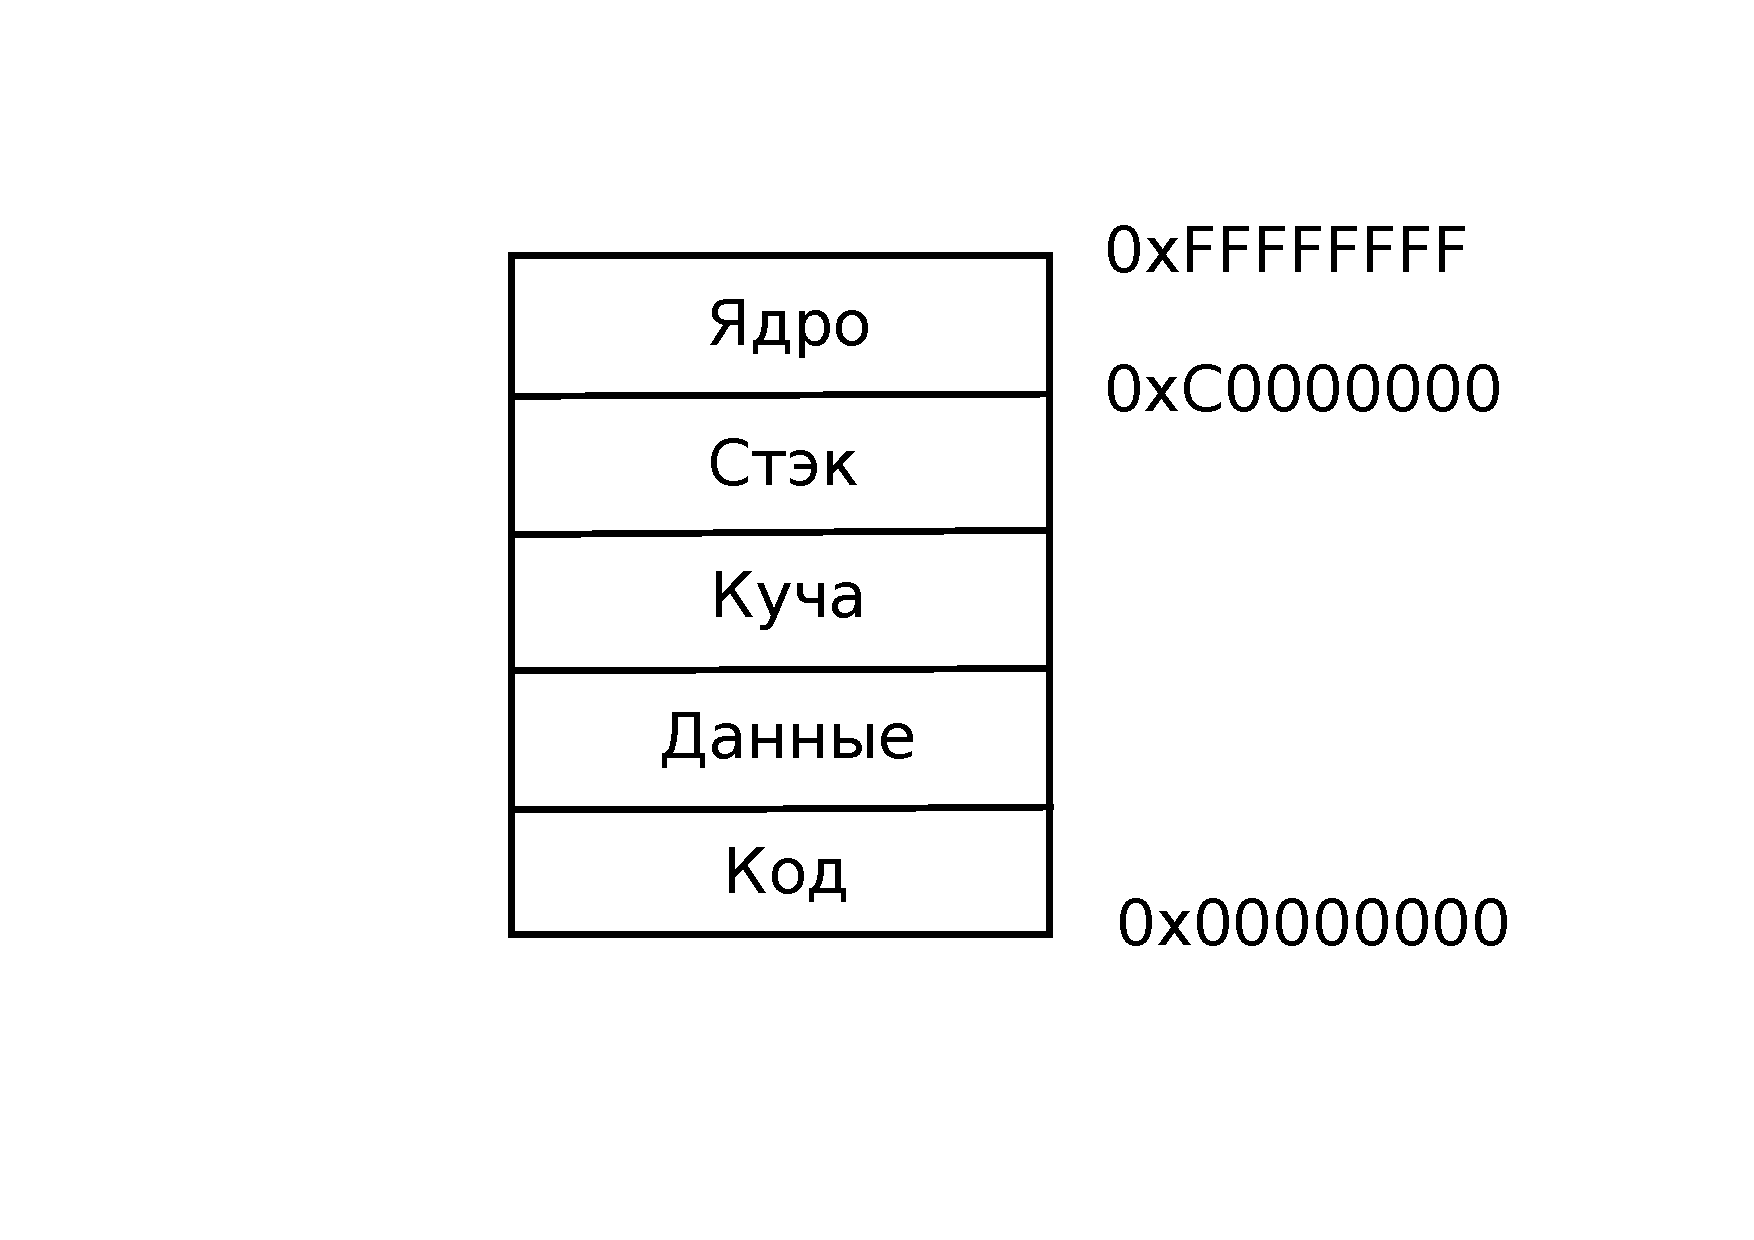
\includegraphics[width=0.99\textwidth]{img/mem_model.pdf}
\end{center}       
\end{frame}

\iframe{Выделение памяти} 
	Расширение сегмента данных: 
   \begin{lstlisting}
int brk(void *endds); 
void *sbrk(intptr_t incr); \end{lstlisting}

	\vspace{0.4em} Выделение новых сегментов из анонимной памяти: 
   \begin{lstlisting}
void *mmap(
   void *addr,
   size_t len,
   int prot, 
   int flags,
   int fildes,
   off_t off
); \end{lstlisting}
\end{frame}

\iframe{Утилита pmap(1)} 
\lstinputlisting[language=C]{listings/sl52.c}
\end{frame}

\iframe{Процесс} 
	Процесс -- это совокупность программы и метаинформации, описывающей её выполнение \textcopyright KorG

	\vspace{1em} Выполняются параллельно и формально независимы друг от друга
\end{frame}

\iframe{Состояния процесса} 
\begin{center}
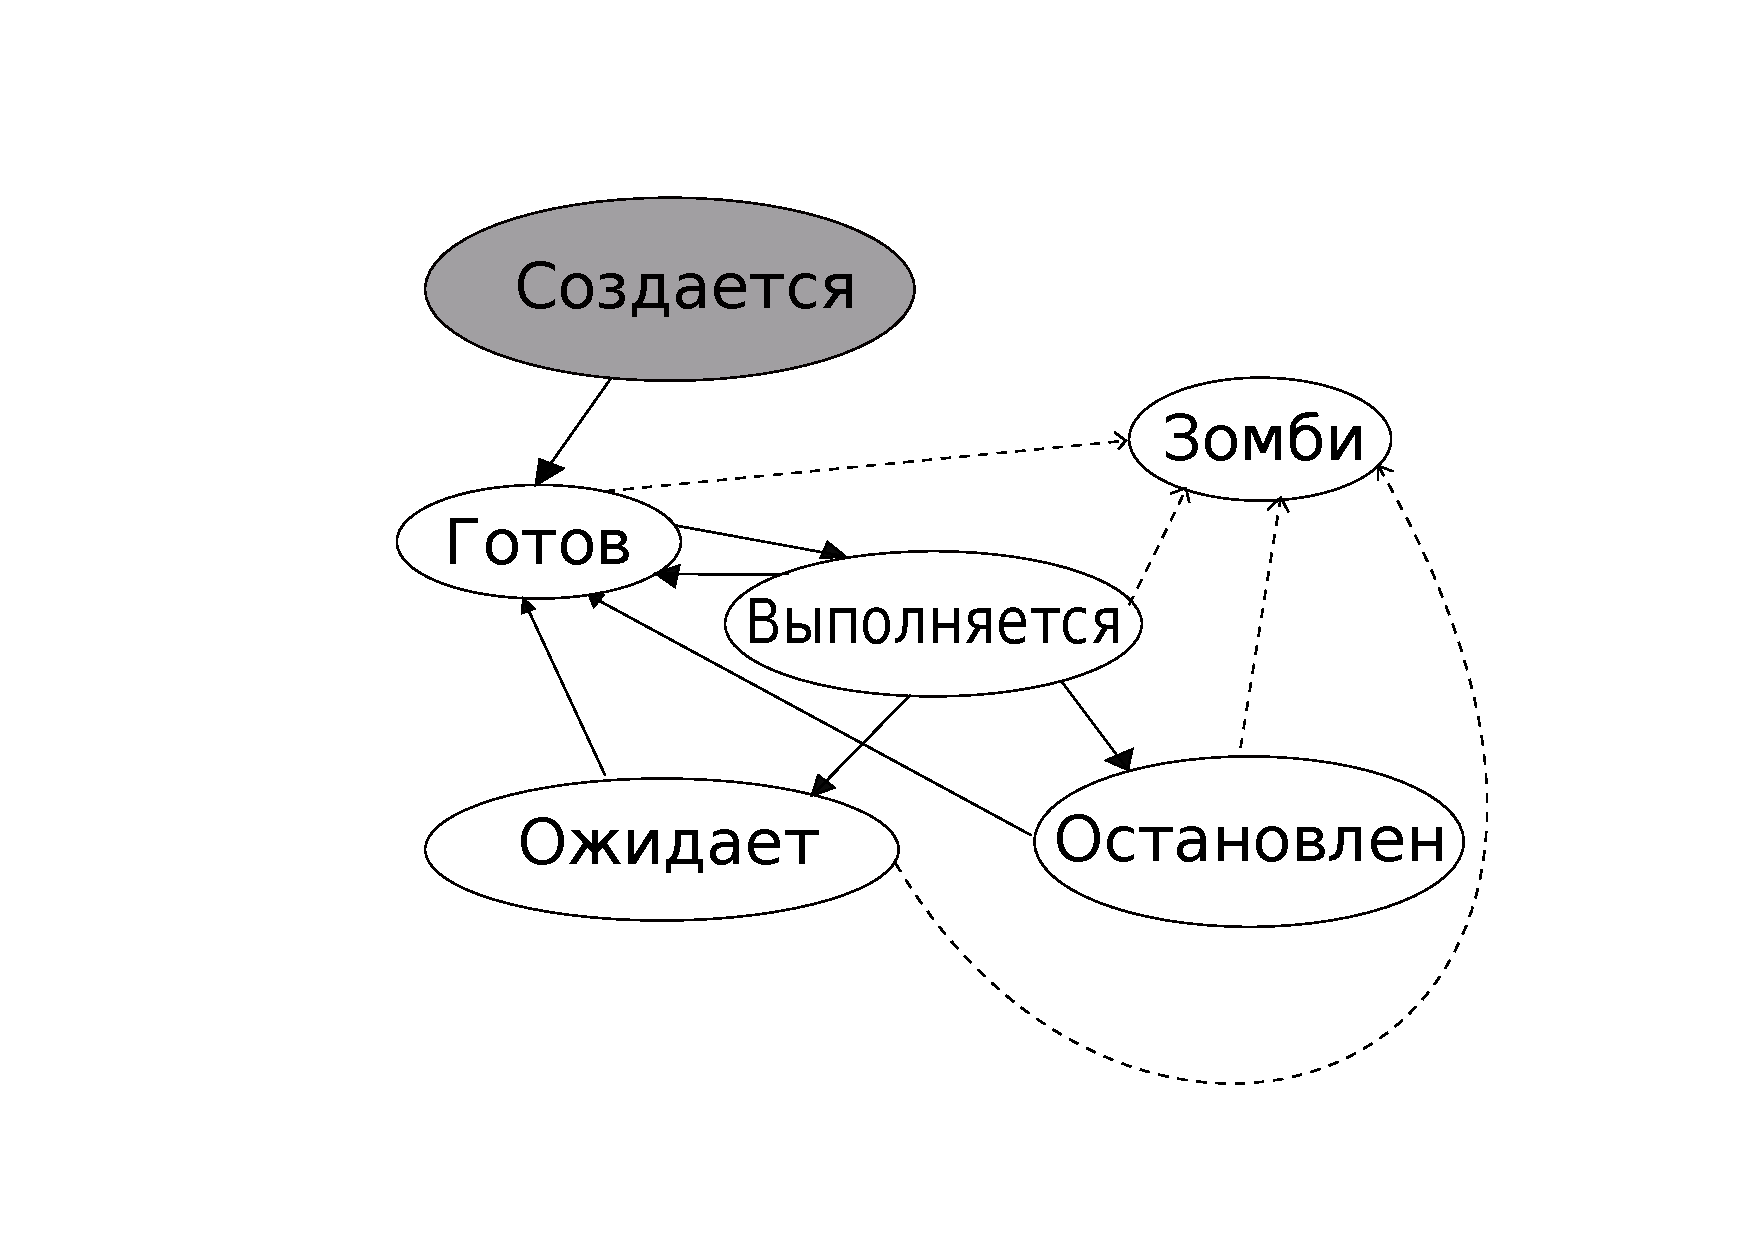
\includegraphics[width=0.99\textwidth]{img/process_states.pdf}
\end{center}      
\end{frame}

% vim: ft=tex cc=79 ts=3 sw=3 et
% 
\pframe{Благодарности}

\begin{itemize}
\item Афанасьев Дмитрий Борисович
\item Горская Александра Андреевна
\item Ховалкина Ксения Николаевна
\item Киреев Валерий Юрьевич
\item и многие другие...
\end{itemize}

\end{frame}
 % благодарности
%%%%%%%%%%%%%%%%%%%%%%%%%%%%%%%%%%%%%%%%%%%%%%%%%%%%%%%%%%%%%%%%%%%%%%%%%%%%%%%
\usebackgroundtemplate{}
\begin{frame}[fragile]
   \vspace{3em}
   \centering \LARGE Спасибо за внимание

   \vspace{4em}
   \begin{tabular}{c}
      \begin{lstlisting}[basicstyle=\tiny]
      # perl '-es!!),-#(-.?{<>-8#=..#<-*}>;*7-86)!;y!#()-?{}!\x20/`-v;<!;s++$_+ee'
      \end{lstlisting} 
   \end{tabular}
\end{frame}

\end{document}
